\chapter{Sharding} 
Sharding là một phương pháp phân phối dữ liệu trên nhiều máy. MongoDB sử dụng sharding để hỗ trợ triển khai với các tập dữ liệu rất lớn và các hoạt động thông lượng cao.

Các hệ thống cơ sở dữ liệu với các tập dữ liệu lớn hoặc các ứng dụng thông lượng cao có thể thách thức khả năng của một máy chủ đơn lẻ. Ví dụ, tỷ lệ truy vấn cao có thể làm cạn kiệt dung lượng CPU của máy chủ. Các kích thước bộ làm việc lớn hơn RAM của hệ thống làm tăng dung lượng I / O của ổ đĩa.

Có hai phương pháp để giải quyết sự tăng trưởng hệ thống: mở rộng theo chiều dọc và chiều ngang.

Chia tỷ lệ theo chiều dọc liên quan đến việc tăng dung lượng của một máy chủ đơn lẻ, chẳng hạn như sử dụng CPU mạnh hơn, tăng thêm RAM hoặc tăng dung lượng bộ nhớ. Các hạn chế trong công nghệ có sẵn có thể hạn chế một máy duy nhất không đủ mạnh cho một khối lượng công việc đã cho. Ngoài ra, các nhà cung cấp dựa trên đám mây có trần cứng dựa trên các cấu hình phần cứng có sẵn. Kết quả là, có tối đa thực tế cho việc mở rộng theo chiều dọc.

Chia tỷ lệ theo chiều ngang liên quan đến việc chia bộ dữ liệu hệ thống và tải trên nhiều máy chủ, thêm máy chủ bổ sung để tăng dung lượng theo yêu cầu. Mặc dù tốc độ hoặc dung lượng tổng thể của một máy đơn có thể không cao, mỗi máy sẽ xử lý một tập hợp con của khối lượng công việc tổng thể, có khả năng mang lại hiệu quả tốt hơn so với một máy chủ dung lượng cao tốc độ cao duy nhất. Việc mở rộng khả năng triển khai chỉ yêu cầu thêm các máy chủ bổ sung nếu cần, có thể thấp hơn tổng chi phí so với phần cứng cao cấp cho một máy. Cân  sự phức tạp trong cơ sở hạ tầng và bảo trì cho việc triển khai.

MongoDB hỗ trợ mở rộng theo chiều ngang thông qua sharding.

\section{Sharded Cluster}
Một cụm MongoDB shard bao gồm các thành phần sau:

\begin{itemize}
\item shard: Mỗi shard chứa một tập con của dữ liệu được shard. Mỗi shard có thể được triển khai như một bộ bản sao.
\item mongos: Các mongos hoạt động như một bộ định tuyến truy vấn, cung cấp một giao diện giữa các ứng dụng máy khách và cụm shard.
\item máy chủ cấu hình: Máy chủ cấu hình lưu trữ cài đặt siêu dữ liệu và cấu hình cho cụm. Theo MongoDB 3.4, các máy chủ cấu hình phải được triển khai như một bộ bản sao (CSRS).
\end{itemize}
Đồ họa sau đây mô tả sự tương tác của các thành phần trong một cụm shard:

\begin{figure}[h!]
\centering
\captionsetup{justification=centering,margin=1cm}
  	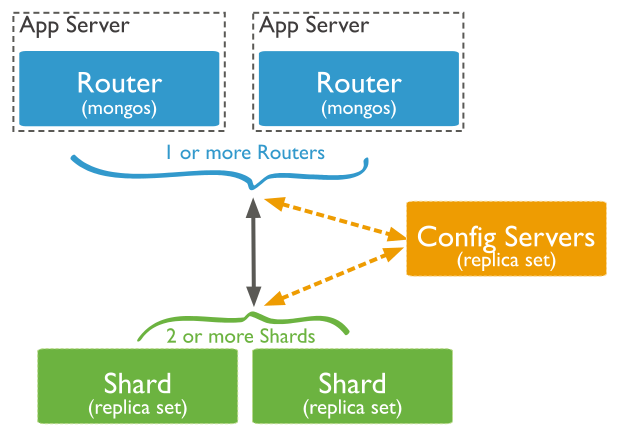
\includegraphics[scale=1]{sharded-cluster-production-architecture.bakedsvg.svg}
  \caption{Sơ đồ của một cụm mẫu shard cho mục đích sản xuất. Chứa chính xác 3 máy chủ cấu hình, 2 hoặc nhiều bộ định tuyến truy vấn $`mongos`$ và ít nhất 2 mảnh. Các mảnh là bộ bản sao.}
  \end{figure}

MongoDB phân chia dữ liệu ở cấp thu thập, phân phối dữ liệu thu thập trên các shard trong cụm.

\section{Shard Keys}
Để phân phối các tài liệu trong một bộ sưu tập, MongoDB phân vùng bộ sưu tập bằng cách sử dụng khóa shard. Khóa shard bao gồm một trường hoặc trường bất biến tồn tại trong mọi tài liệu trong bộ sưu tập đích.

Bạn chọn khoá shard khi sharding một bộ sưu tập. Không thể thay đổi khóa shard sau khi sharding. Bộ sưu tập được phân loại có thể chỉ có một khóa shard. 

Để shard một bộ sưu tập không trống, bộ sưu tập phải có chỉ mục bắt đầu bằng khóa shard. Đối với các bộ sưu tập rỗng, MongoDB tạo chỉ mục nếu bộ sưu tập không có chỉ mục thích hợp cho khóa shard đã chỉ định. 

Sự lựa chọn của shard key ảnh hưởng đến hiệu suất, hiệu quả và khả năng mở rộng của một cluster bị phân mảnh. Một cụm với phần cứng và cơ sở hạ tầng tốt nhất có thể bị tắc nghẽn bởi sự lựa chọn của khóa shard. Việc lựa chọn mã khóa và chỉ số sao lưu của nó cũng có thể ảnh hưởng đến chiến lược tích trữ mà cụm của bạn có thể sử dụng.

\section{Chunk}
Các phân vùng MongoDB phân chia dữ liệu thành các đoạn. Mỗi đoạn có một cận trên và dưới dựa trên khoá shard.

MongoDB di chuyển các đoạn trên các mảnh trong cluster bị phân mảnh bằng cách sử dụng cân bằng cluster bị phân mảnh. Các cân bằng cố gắng để đạt được một sự cân bằng thậm chí của khối trên tất cả các mảnh trong cụm.

\section{Ưu điểm của Sharding}
\paragraph{Đọc / ghi}
MongoDB phân phối khối lượng công việc đọc và ghi trên các shard trong cụm shard, cho phép mỗi shard xử lý một tập con của các phép toán cụm. Cả hai khối lượng công việc đọc và ghi có thể được thu nhỏ theo chiều ngang trên cụm bằng cách thêm nhiều shard hơn.

Đối với các truy vấn bao gồm khóa shard hoặc tiền tố của khóa shard phức hợp, mongos có thể nhắm mục tiêu truy vấn tại shard cụ thể hoặc tập hợp các shard. Các hoạt động được nhắm mục tiêu này thường hiệu quả hơn là phát sóng tới mọi shard trong cụm.

\paragraph{Khả năng lưu trữ}
Sharding phân phối dữ liệu trên các shard trong cụm, cho phép mỗi shard chứa một tập hợp con của tổng số dữ liệu cụm. Khi tập dữ liệu phát triển, các shard bổ sung sẽ tăng dung lượng lưu trữ của cụm.

\paragraph{Tính sẵn sàng cao}
Một cụm shard có thể tiếp tục thực hiện một phần hoạt động đọc / ghi ngay cả khi một hoặc nhiều shard không có sẵn. Mặc dù tập hợp con dữ liệu trên các shard không có sẵn không thể truy cập được trong thời gian ngừng hoạt động, nhưng việc đọc hoặc viết trực tiếp tại các shard có sẵn vẫn có thể thành công.

Trong môi trường sản phẩm, shard cá nhân nên được triển khai dưới dạng bản sao, cung cấp khả năng dự phòng và tính khả dụng cao hơn.

\section{Cân nhắc trước khi Sharding}
Yêu cầu cơ sở hạ tầng cụm phức tạp và yêu cầu phức tạp đòi hỏi phải lập kế hoạch, thực hiện và bảo trì cẩn thận.

Cân nhắc cẩn thận trong việc chọn khóa shard là cần thiết để đảm bảo hiệu suất và hiệu quả của cụm. Bạn không thể thay đổi khóa shard sau khi sharding, cũng không thể unshard một bộ sưu tập sharded. Xem Chọn một khóa shard.

Sharding có một số yêu cầu và hạn chế hoạt động nhất định. Xem các hạn chế hoạt động trong các cụm đã shard để biết thêm thông tin.

Nếu các truy vấn không bao gồm khóa shard hoặc tiền tố của khóa shard hợp chất, mongos thực hiện một hoạt động phát sóng, truy vấn tất cả các shard trong cụm bị phân mảnh. Các truy vấn phân tán / thu thập này có thể là các hoạt động chạy dài.

\section{Sharded and Non-Sharded Collections}
Một cơ sở dữ liệu có thể có một hỗn hợp các bộ sưu tập bị phân mảnh và không bị trầy xước. Các bộ sưu tập được phân chia được shard và phân phối trên các shard trong cụm. Bộ sưu tập chưa được lưu trữ được lưu trữ trên shard chính. Mỗi cơ sở dữ liệu có shard chính của riêng nó.

\begin{figure}[h!]
\centering
\captionsetup{justification=centering,margin=1cm}
  	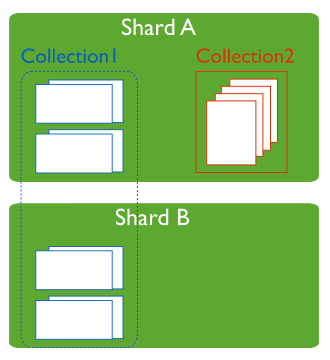
\includegraphics[scale=1]{sharded-cluster-primary-shard.bakedsvg.svg}
  \caption{Sơ đồ shard chính. Phân đoạn chính chứa các bộ sưu tập không bị shard cũng như các khối tài liệu từ các bộ sưu tập được phân loại. Shard A là shard chính.}
  \end{figure}

\section{Kết nối với một cụm được shard}
Bạn phải kết nối với bộ định tuyến mongos để tương tác với bất kỳ bộ sưu tập nào trong cụm được shard. Điều này bao gồm các bộ sưu tập bị phân tán và không bị trói buộc. Khách hàng không bao giờ nên kết nối với một mảnh duy nhất để thực hiện các hoạt động đọc hoặc ghi.

\begin{figure}[h!]
\centering
\captionsetup{justification=centering,margin=1cm}
  	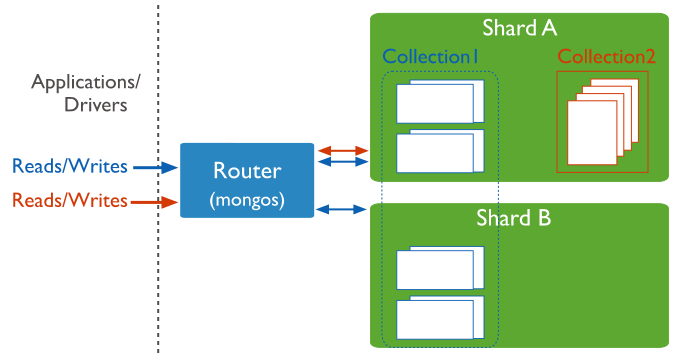
\includegraphics[scale=1]{sharded-cluster-mixed.bakedsvg.svg}
  \caption{Sơ đồ các ứng dụng / trình điều khiển đưa ra các truy vấn tới mongos cho bộ sưu tập không bị quản lý cũng như bộ sưu tập được phân loại. Máy chủ cấu hình không được hiển thị. Bạn có thể kết nối với một mongos giống như cách bạn kết nối với một Mongod, chẳng hạn như thông qua trình bao mongo hoặc trình điều khiển MongoDB.}
  \end{figure}

Bạn có thể kết nối với một mongos giống như cách bạn kết nối với một Mongod, chẳng hạn như thông qua trình bao mongo hoặc trình điều khiển MongoDB.

\section{Sharding Strategy}
MongoDB hỗ trợ hai chiến lược sharding để phân phối dữ liệu trên các cụm bị phân mảnh.

\paragraph{Hashed Sharding}
Hashed Sharding liên quan đến việc tính toán giá trị băm của giá trị của trường khóa. Mỗi đoạn sau đó được gán một phạm vi dựa trên các giá trị khóa shard băm.

\begin{figure}[h!]
\centering
\captionsetup{justification=centering,margin=1cm}
  	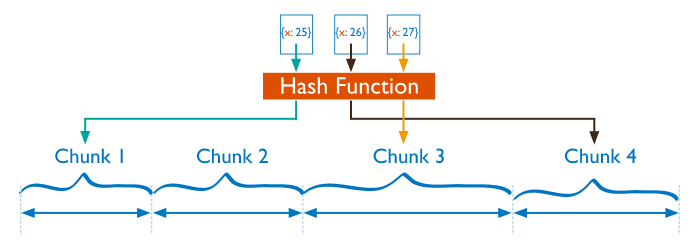
\includegraphics[scale=1]{sharding-hash-based.bakedsvg.svg}
  \caption{Sơ đồ shard dựa trên băm.}
  \end{figure}

Mặc dù một loạt các khóa shard có thể là “đóng”, nhưng các giá trị băm của chúng không thể ở cùng một đoạn. Phân phối dữ liệu dựa trên các giá trị băm tạo điều kiện phân phối dữ liệu thậm chí nhiều hơn, đặc biệt là trong các tập dữ liệu trong đó khóa phân tử thay đổi một cách đơn điệu.

Tuy nhiên, phân phối băm có nghĩa là các truy vấn dựa trên phạm vi trên khóa shard ít có khả năng nhắm mục tiêu một shard đơn lẻ, dẫn đến nhiều hoạt động phát rộng hơn theo cụm

\paragraph{Ranged Sharding}
Sự phân rã có phạm vi liên quan đến việc chia dữ liệu thành các phạm vi dựa trên các giá trị khóa shard. Mỗi đoạn sau đó được gán một phạm vi dựa trên các giá trị khóa shard.

\begin{figure}[h!]
\centering
\captionsetup{justification=centering,margin=1cm}
  	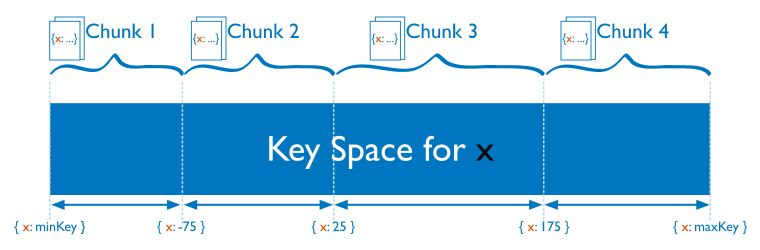
\includegraphics[scale=1]{sharding-range-based.bakedsvg.svg}
  \caption{Sơ đồ không gian giá trị khóa shard được chia thành các phạm vi hoặc khối nhỏ hơn.}
  \end{figure}

Một loạt các khóa shard có giá trị “đóng” có nhiều khả năng cư trú trên cùng một đoạn. Điều này cho phép các hoạt động được nhắm mục tiêu như một mongos có thể định tuyến các hoạt động đến chỉ các mảnh có chứa dữ liệu cần thiết.

Hiệu quả của sharding dao động phụ thuộc vào phím shard được chọn. Các khóa shard kém được xem là có thể dẫn đến phân phối dữ liệu không đồng đều, có thể phủ nhận một số lợi ích của việc tích trữ hoặc có thể gây ra tắc nghẽn hiệu suất.

\section{Zones in Sharded Clusters}
Trong các cụm shard, bạn có thể tạo các vùng dữ liệu được phân loại dựa trên khóa shard. Bạn có thể kết hợp từng vùng với một hoặc nhiều mảnh trong cụm. Phân đoạn có thể kết hợp với bất kỳ số vùng nào. Trong một cụm cân bằng, MongoDB di chuyển các khối được bao phủ bởi một vùng chỉ cho các mảnh vỡ liên kết với vùng đó.

Mỗi vùng bao gồm một hoặc nhiều dải giá trị khóa shard. Mỗi phạm vi một vùng bao gồm luôn luôn bao gồm ranh giới thấp hơn của nó và độc quyền của ranh giới trên của nó.

\begin{figure}[h!]
\centering
\captionsetup{justification=centering,margin=1cm}
  	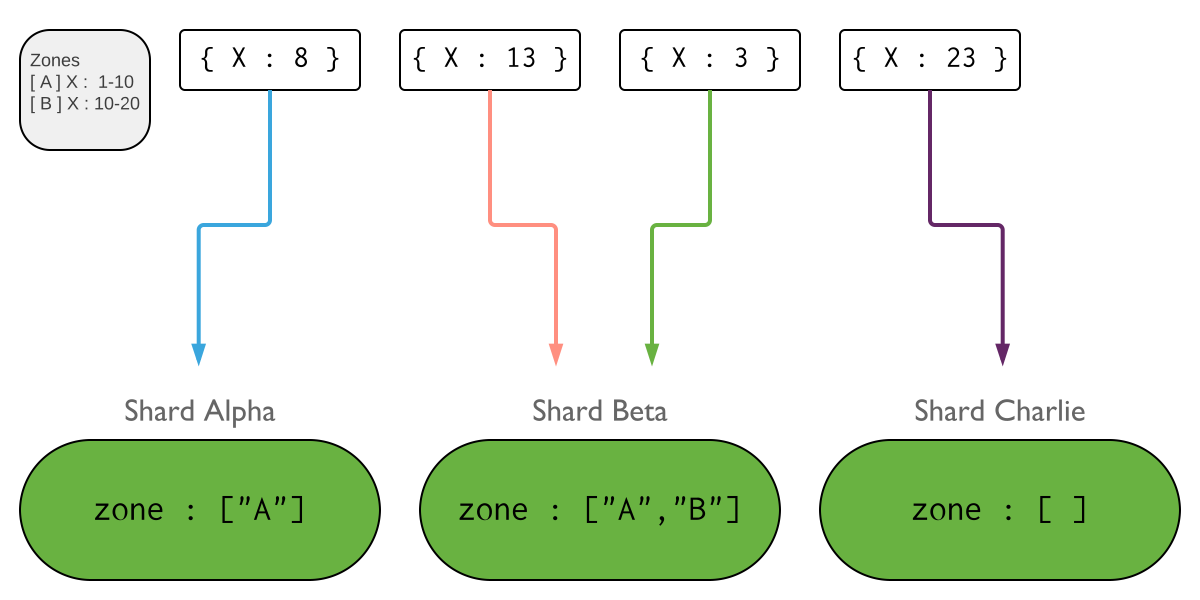
\includegraphics[scale=1]{sharded-cluster-zones.bakedsvg.svg}
  \caption{Sơ đồ phân bố dữ liệu dựa trên các vùng trong một cụm shard}
  \end{figure}

Bạn phải sử dụng các trường có trong khóa shard khi xác định phạm vi mới cho vùng cần bao gồm. Nếu sử dụng khóa shard hợp chất, phạm vi phải bao gồm tiền tố của khóa shard. 

Khi chọn một khóa shard, hãy xem xét cẩn thận khả năng sử dụng sharding khu vực trong tương lai, vì bạn không thể thay đổi khóa shard sau khi sharding bộ sưu tập.

Phổ biến nhất, các khu vực phục vụ để cải thiện địa phương của dữ liệu cho các cụm shard trải rộng trên nhiều trung tâm dữ liệu.

\section{Collations in Sharding}
Sử dụng lệnh shardCollection với đối chiếu: tùy chọn ${locale: "simple"}$ để phân tích một bộ sưu tập có collation mặc định. Sharding thành công đòi hỏi rằng:
\begin{itemize}
\item Bộ sưu tập phải có chỉ mục có tiền tố là khóa shard
\item Chỉ mục phải có collation ${locale: "simple"}$
\end{itemize}
Khi tạo bộ sưu tập mới với collation, đảm bảo các điều kiện này được đáp ứng trước khi sharding bộ sưu tập.